\section*{Appendix}
\label{sec:appendix}

\section{실험 세부사항}
\label{app:experimental_setups}

\subsection{Data Preparation}
Mathematical reasoning tasks의 경우, 표준 protocol~\cite{zhao2025d1,ou2025principled}을 따라 각 dataset의 official training split으로 학습한다.
Code generation tasks의 경우, AceCoder-87K dataset~\cite{zeng2025acecoder}을 채택한다. DiffuCoder~\cite{gong2025diffucoder}의 data processing pipeline을 따라, 검증 가능한 unit tests가 갖춰진 AceCoder-87K의 challenging samples 21K개를 추가로 선택한다.

\subsection{Training Configuration}
우리의 training setup은 대체로~\cite{huang2025reinforcing}를 따른다.
\cite{huang2025reinforcing}와 달리, 우리는 추가 trainable modules를 도입하지 않고 dLLM에 직접 reinforcement learning을 수행한다.
Rollout phase 동안에는 exact autoregressive sampling을 채택하며, 이는 표준 GRPO formulation 아래 직접적인 log-probability 계산을 가능하게 한다.
또한 JustGRPO가 빠르고 안정적인 convergence를 보이므로 training steps의 총수도 줄인다.
모든 실험은 16$\times$ NVIDIA H100 GPUs에서 수행된다. 자세한 hyperparameters는 Table~\ref{tab:hyperparams}에 보고한다.


\begin{table}[H]
    \centering
    \caption{JustGRPO의 \textbf{training hyperparameters}\protect\footnotemark{}.}
    \label{tab:hyperparams}
    \begin{tabular}{lc}
        \toprule
        \textbf{Hyperparameter} & \textbf{Value} \\
        \midrule
        Base Model & LLaDA 8B Instruct \\
        RL Algorithm & GRPO \\
        Optimizer & AdamW \\
        Learning Rate & $5 \times 10^{-6}$ \\
        LR Scheduler & Constant \\
        Weight Decay & 0.0 \\
        Optimizer Betas $(\beta_1, \beta_2)$ & $(0.9, 0.999)$ \\
        Global Batch Size & 64 \\
        Group Size ($G$) & 16 \\
        Policy Update Steps & 1 \\
        Training Steps & 125 \\
        Max Completion Length & 256 \\
        Sampling Temperature & 1.0 \\
        KL Penalty Coefficient & 0.0 \\
        \bottomrule
    \end{tabular}
\end{table}

\footnotetext{경험적으로 GSM8K는 훨씬 더 빠르게 convergence한다(약 50 steps에서 이미 $\sim$89\% accuracy에 도달). 반면 coding tasks(HumanEval, MBPP)는 더 느리며 전체 125 steps의 이점을 얻는다. 따라서 일관성을 위해 모든 datasets에 대해 125 steps를 동일하게 사용했다.
}
\subsection{Reward Function}
\label{app:reward_function}

\paragraph{Mathematical Reasoning Tasks.}
우리는 binary reward scheme을 사용한다. 각 completion은~\cite{huang2025reinforcing}를 따라 final answer가 ground-truth solution과 수학적으로 동등할 때에만 1의 reward를 받는다.

\paragraph{Code Generation Tasks.}
Code generation의 경우, total reward $r$은 correctness reward $r_{\text{code}}$와 format reward $r_{\text{format}}$의 합으로 정의된다.
\begin{equation}
    r = r_{\text{code}} + r_{\text{format}}.
\end{equation}

\begin{itemize}
    \item \textbf{Correctness reward ($r_{\text{code}}$)}: 제공된 unit tests에서 생성된 code의 pass rate(0에서 1 사이)로 정의된다. 이 항은 $r_{\text{format}} = 1$일 때에만 평가된다.
    \item \textbf{Format reward ($r_{\text{format}}$)}: 문법적으로 유효한 outputs을 장려하도록 설계된 heuristic reward이다.
    \begin{itemize}
        \item $1.0$: 올바른 Python syntax를 가진 유효한 Markdown code block.
        \item $0.5$: Syntax errors를 포함하지만 유효한 Markdown code block.
        \item $0.0$: 유효한 Markdown code block 생성 실패.
    \end{itemize}
\end{itemize}


\section{Reasoning Boundary에 대한 추가 분석 결과}
\label{app:boundary_ablations}
Section~\ref{sec:rethink_value_of_AO}에서 제시한 reasoning boundary에 관한 발견의 robust성을 추가로 검증하기 위해, LLaDA-Instruct model~\cite{nie2025large}을 사용하여 HumanEval benchmark에서 확장 분석을 수행한다. Temperature와 sampling strategies가 reasoning performance에 미치는 영향을 조사한다.

\subsection{Temperature Analysis}
\label{app:temperature_analysis}
\begin{figure}[ht]\centering
    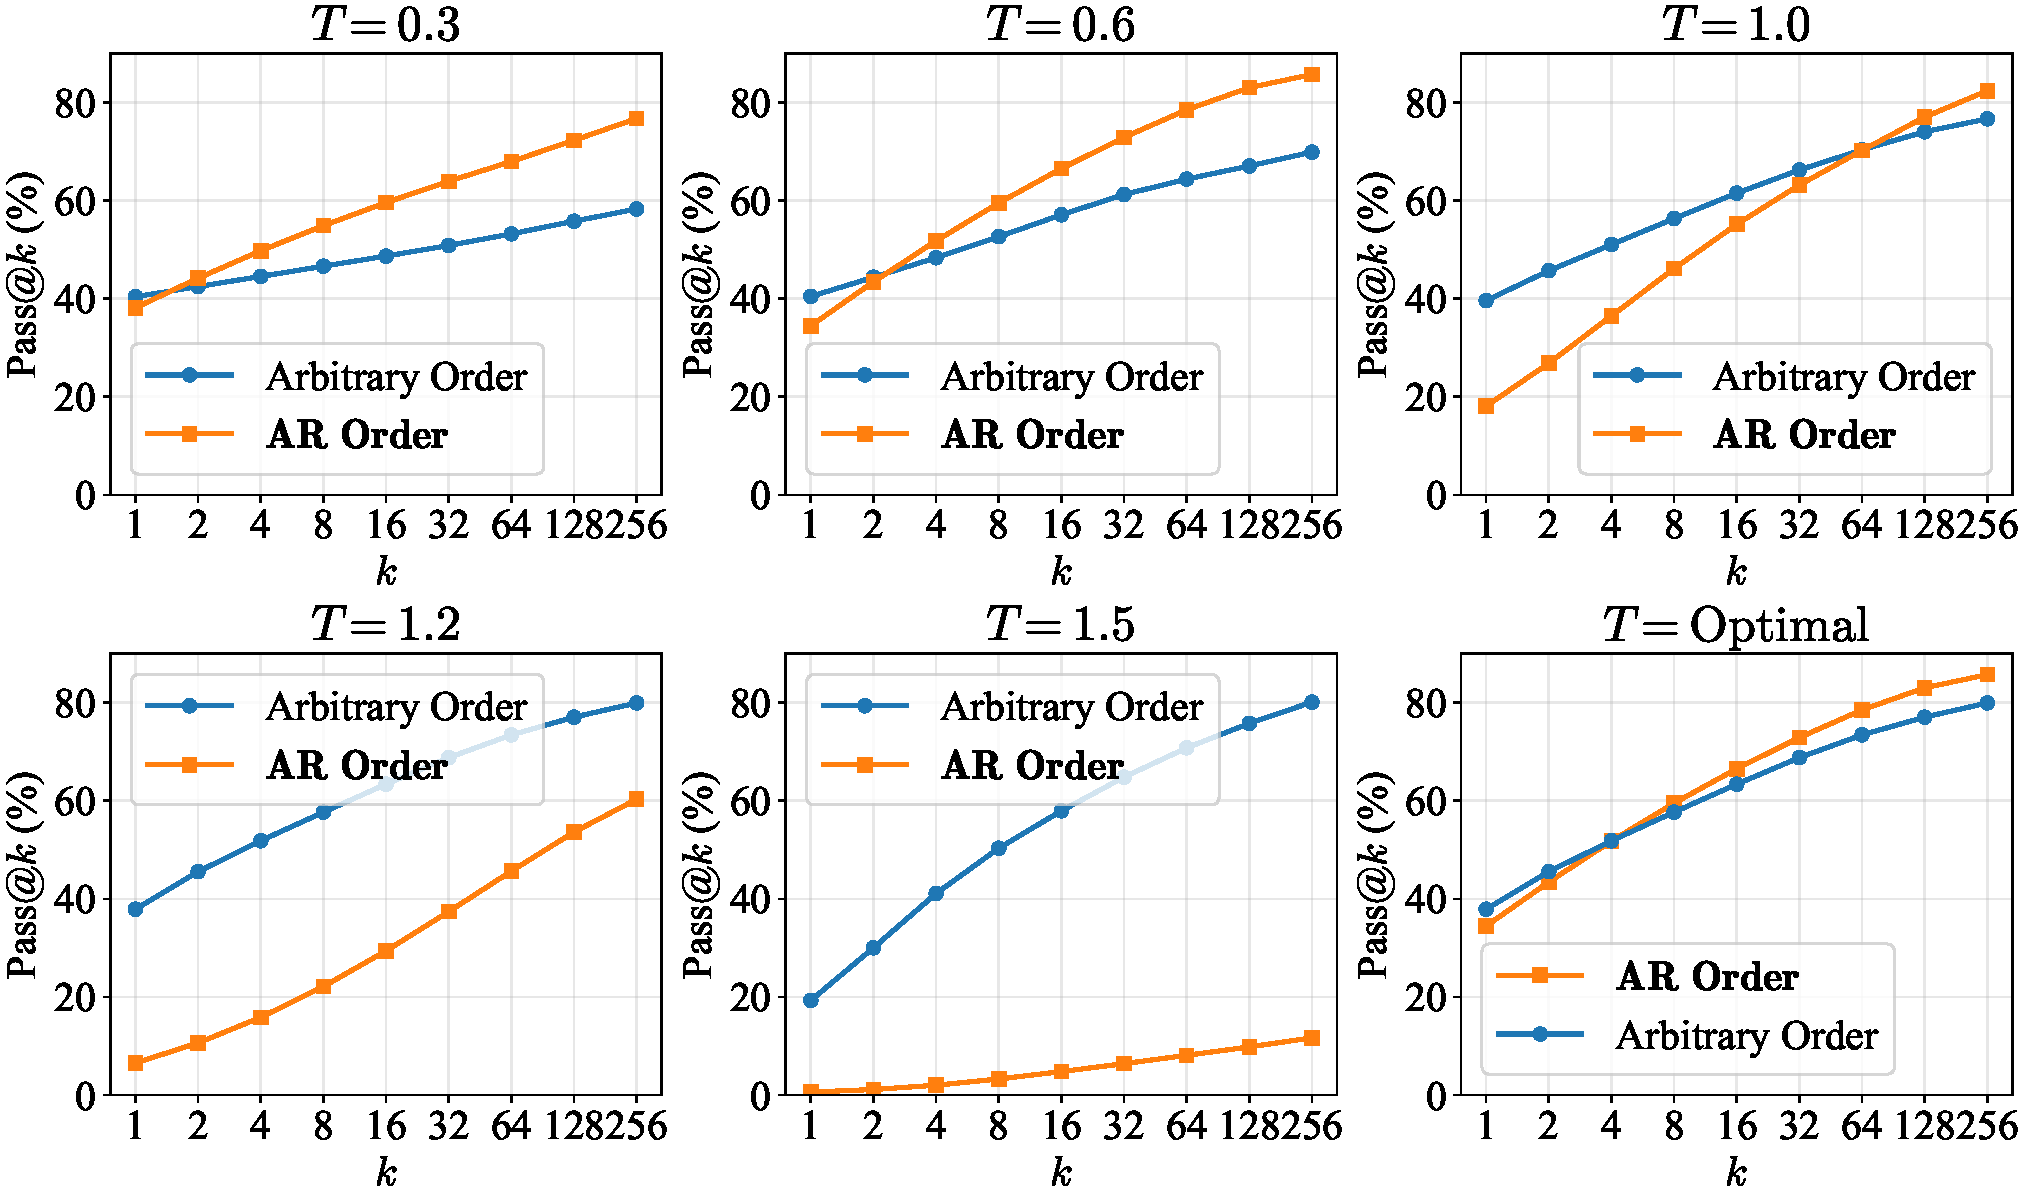
\includegraphics[width=.75\linewidth]{figures/humaneval_temp.pdf}
    \caption{
        \textbf{서로 다른 temperatures에서의 Pass@$k$ comparison\label{fig:passk_comparison_temperature}}.
    }
\end{figure}

HumanEval에서 우리는 Pass@$k$ plot을 $k=256$까지 확장한다. $1.0$에 가까운 temperatures에서는 두 modes 사이의 crossover가 비교적 큰 $k$에서 발생하며, 더 큰 budget은 그 이후의 비교를 검토할 수 있게 한다.
\cref{fig:passk_comparison_temperature}에 보이듯, AR mode는 표준적인 패턴을 보인다. 성능은 moderate temperatures($T \approx 0.6$)에서 peak에 도달하고 $T > 1.0$일 때 저하되는 반면, Arbitrary Order mode는 더 높은 temperatures에서 peak performance를 달성한다.

이 관찰은 Section~\ref{sec:rethink_value_of_AO}에서 논의한 \textit{entropy degradation} 메커니즘과 일치한다. Diffusion sampler가 critical branching points에서 본질적으로 uncertainty를 억제하므로, 충분한 exploration을 유도하려면 더 높은 temperatures가 필요하다.
주목할 점은 이러한 optimized settings에서도 arbitrary order mode가 우리의 실험에서 AR mode의 reasoning potential에 미치지 못한다는 것이다.
\cref{fig:passk_comparison_temperature}의 ``Optimal'' comparison setting(오른쪽 아래)에 나타난 것처럼, best-performing AR configuration은 여전히 optimal arbitrary order baseline보다 더 나은 scaling behavior를 보인다. 그럴듯한 설명은 arbitrary order decoding에서 지나치게 높은 temperatures가 높은 결정성이 필요한 tokens(\eg, code syntax 또는 mathematical suffixes)에 noise를 주입하여 nonsensical outputs과 저하된 결과를 초래한다는 것이다~\cite{wang2025beyond,huang2025low}.

\subsection{Different Sampling Algorithms}
우리는 Figure~\ref{fig:alg_comparison}(a)에서 negative entropy sampling (Neg-Entropy) ~\cite{ye2025dream} 및 top-$k$ margin sampling (Margin) ~\cite{kim2025train} 같은 다양한 sampling algorithms도 실험한다.
\begin{figure}[t]\centering
    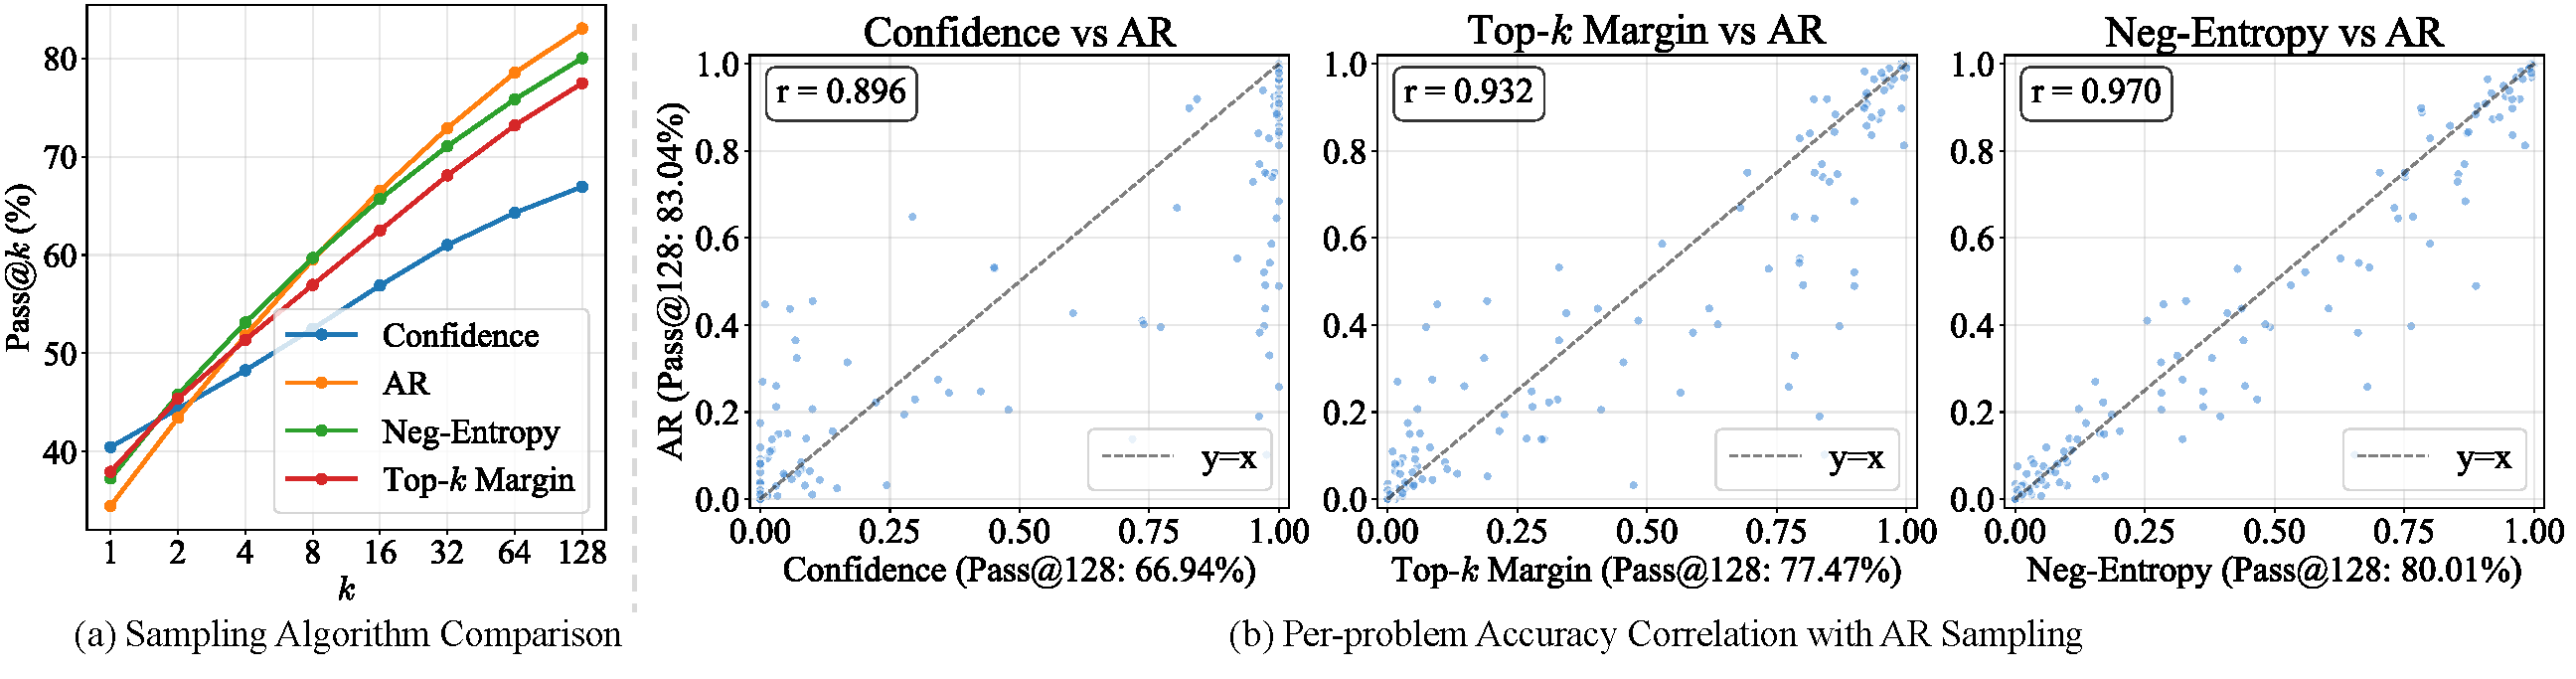
\includegraphics[width=\linewidth]{figures/alg_compare.pdf}
    \caption{
        \textbf{(a) Sampling algorithm comparison}.
        \textbf{(b) 서로 다른 sampling algorithms와 AR 사이의 per-problem accuracy 상관관계}.
        Pass@$k$ 성능이 더 높은 algorithms는 problem-level performance에서 \emph{AR과 더 높은 correlation}을 보이는 경향이 있다.
        \label{fig:alg_comparison}
    }
\end{figure}
결과는 더 정교한 sampling algorithms가 default confidence-based sampling보다 더 나은 Pass@$k$ 성능을 달성할 수는 있지만, 여전히 AR order를 따라잡지는 못함을 보여 준다.
한편 이러한 더 나은 Pass@$k$ algorithms는 confidence-based sampling에 비해 약간 더 낮은 Pass@$1$ 성능도 보이며, 전체 Pass@$k$ curve를 AR order의 Pass@$k$ curve에 더 가깝게 만든다.
이 유사성을 조사하기 위해 서로 다른 sampling algorithms와 AR mode 사이의 per-problem accuracy correlation을 계산한다(Figure~\ref{fig:alg_comparison}(b)).
우리는 더 높은 scaling potential(더 높은 Pass@$128$)을 가진 algorithms가 일관되게 AR과 더 강한 correlation을 보이며, 가장 효과적인 방법(Neg-Entropy)은 $0.970$의 correlation을 달성함을 관찰한다.
이는 더 나은 Pass@$k$를 가진 sampling algorithms가 performance characteristics에서 AR처럼 행동하는 경향이 있음을 시사한다.

\begin{figure}[ht]\centering
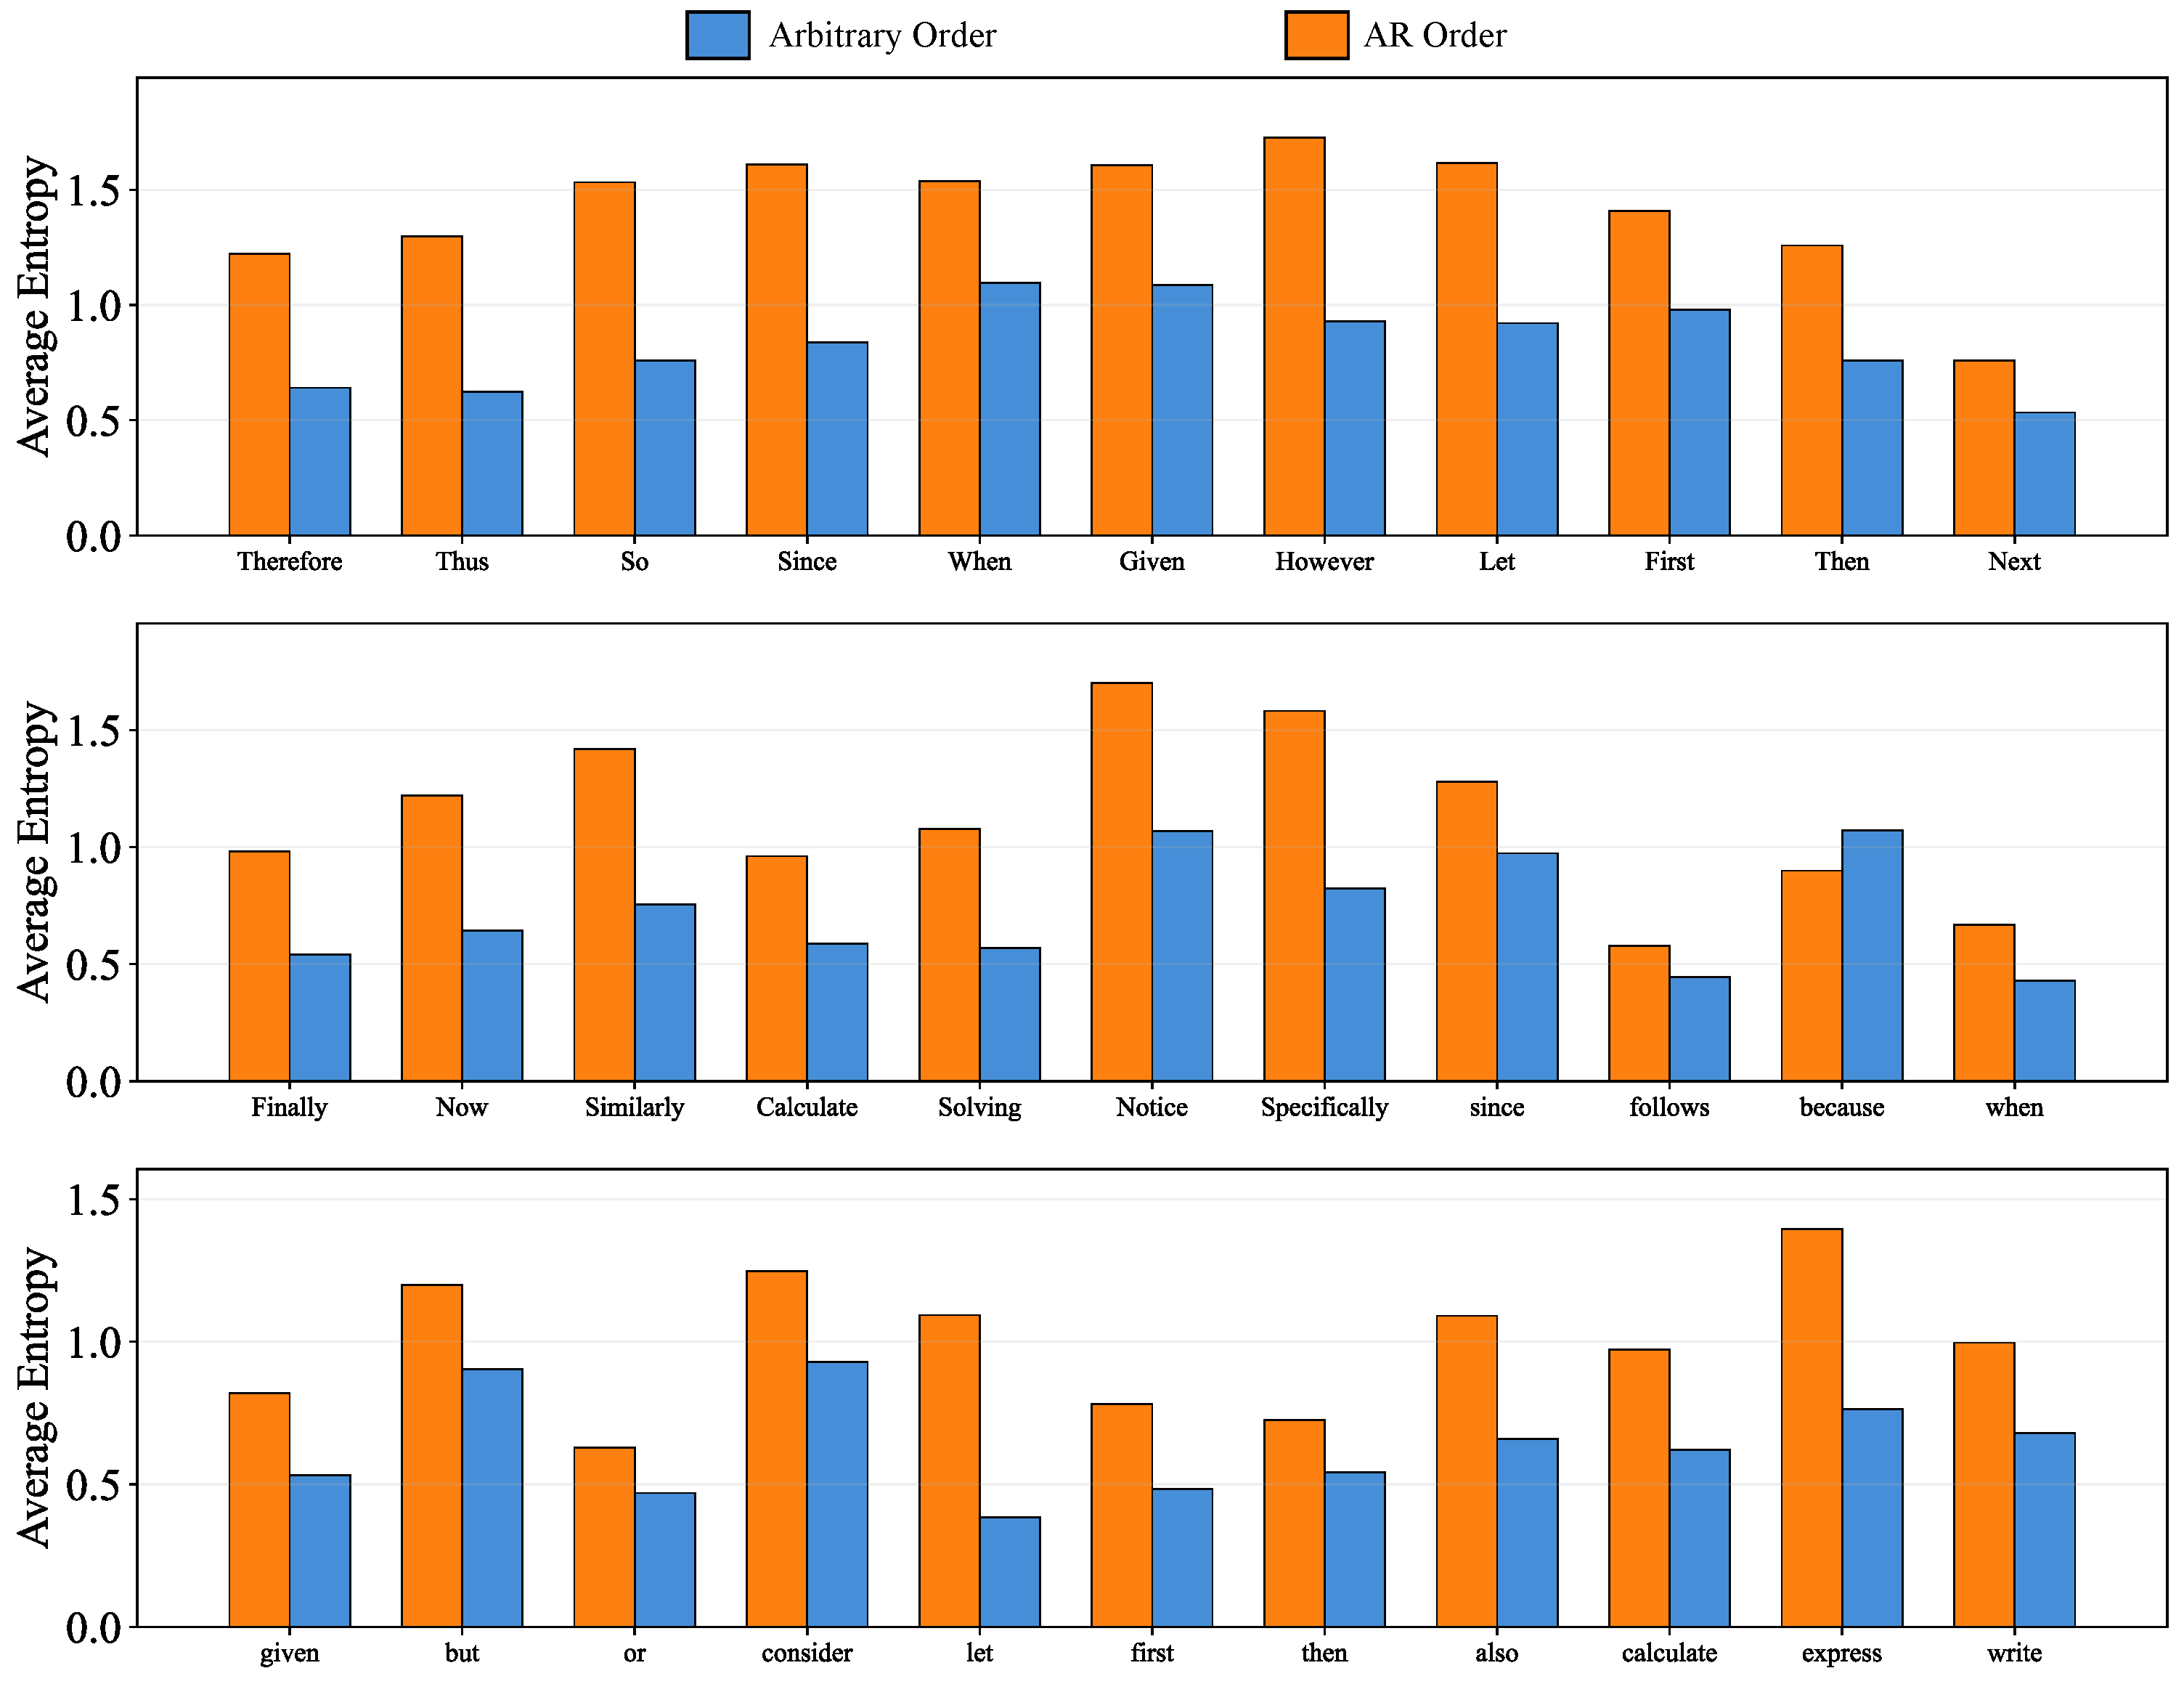
\includegraphics[width=\linewidth]{figures/entropy_bar_compare_more.pdf}
\caption{
    \textbf{더 많은 forking tokens에 대한 entropy comparison results\label{fig:entropy_bar_compare_more}}.
}
\end{figure}

\section{Entropy Degradation에 대한 추가 결과}
\label{app:more_results_entropy_degradation}

Section~\ref{sec:rethink_value_of_AO}에서 관찰한 ``entropy degradation'' 현상의 robust성을 검증하기 위해, 우리는 분석을 더 넓은 범위의 logical connectors로 확장했다. Reasoning chains에서 일반적으로 forking tokens로 작용하는 common connectives의 포괄적인 집합에 대해 실험을 수행했다.

\cref{fig:entropy_bar_compare_more}에 나타난 결과는 이 현상이 이러한 다양한 tokens 전반에서 일관됨을 보여 준다. 주요 발견과 유사하게, AR order는 이러한 forks에서 더 높은 average entropy를 유지하며, 이는 active reasoning과 decision-making을 나타낸다. 반대로 Arbitrary Order는 일관되게 더 낮은 entropy를 낳으며, branching possibilities의 premature collapse와 일치한다.

이 확장 실험에서 평가한 구체적인 forking tokens는 다음을 포함한다. ``Therefore'', ``Thus'', ``So'', ``Since'', ``When'', ``Given'', ``However'', ``Let'', ``First'', ``Then'', ``Next'', ``Finally'', ``Now'', ``Similarly'', ``Calculate'', ``Solving'', ``Notice'', ``Specifically'', ``Follows'', ``Because'', ``But'', ``Or'', ``Consider'', ``Also'', ``Express'', and ``Write''.



\section{Random Order는 대안인가?}
\label{app:random_order}

Section~\ref{sec:rethink_value_of_AO}의 우리의 주요 분석은 dLLM이 실제로 사용되는 방식, 즉 confidence-based sampling과 semi-autoregressive sampling~\cite{nie2025large,zhao2025d1}에 의해 decoding이 구동되는 설정에 관한 것이다. 이것이 bypassing이 발생하고 entropy가 degradation되는 설정이며, 우리의 분석이 겨냥하는 설정이다.

그러나 dLLM이 반드시 그러한 sampler를 사용해야 하는 것은 아니다. 자연스러운 질문은 original dLLM formulation~\cite{mdlm,shi2024simplified}과 연결되는 random decoding order가 다르게 행동할지 여부이다. 우리는 그것 역시 도움이 되지 않음을 발견한다.

\paragraph{Random order does not help coverage, and it breaks generation.}
Pass@$128$에서 random order는 기껏해야 confidence-based sampling과 비슷하며, 여전히 AR order에는 크게 못 미친다(Table~\ref{tab:random_passk}, 위). Pass@$1$은 훨씬 더 나빠서 두 baselines보다도 훨씬 낮다(Table~\ref{tab:random_passk}, 아래). 이유는 간단하다. dLLM에서 각 token은 주변 context로부터 예측되지만, random order는 종종 그 context가 존재하기 전에 모델이 token을 결정하도록 요구한다. 예를 들어 token~1만 알려진 상태에서 token~30을 예측하는 식이다. 그 결과 output은 단순히 틀리는 데 그치지 않고, 다음 LLaDA rollout이 보여 주듯 구조적으로 깨진다.

\begin{quote}
    \small\ttfamily
    3. **Third Month:**\\
    \ - The number of downloads reduced by 30\% compared to the second month.\\
    \ \textbackslash[ 180 - (\ \ \ \textbackslash times 180 - (\ \ \ - 180) = 180 - 0.30 \textbackslash times 180 = 54 \ldots \textbackslash]
\end{quote}

LaTeX가 손상되어 dangling operators와 missing operands가 생긴다. 이런 종류의 outputs은 reward를 얻는 경우가 드물며, 이는 RL이 학습할 수 있는 것을 제한한다.

\paragraph{Random order does not survive RL either.}
그 다음 random order를 우리의 training setup으로 가져온다. JustGRPO와 유사한 exact likelihood factorization을 적용하기 위해, 단일 random permutation을 채택하고 training 내내 고정한다. 우리는 이 variant를 JustGRPO-Random이라 부른다. Pipeline의 나머지는 그대로 유지했을 때, JustGRPO-Random은 GSM8K에서 82.2\%에만 도달하며, AR order의 89.1\%와 비교된다(Table~\ref{tab:random_order_ablation}). 따라서 random order는 remedy로 보이지 않는다. 우리의 실험에서 이는 sampler로서 coverage를 넓히지도 못하고 RL 이후 강한 reasoning을 제공하지도 못한다.

\begin{table}[H]
    \centering
    \caption{\textbf{Random order는 coverage를 개선하지 못하고 single-shot accuracy를 붕괴시킨다.} LLaDA-Instruct에서 측정한 confidence-based arbitrary order, fully random order, AR order의 Pass@$128$(위) 및 Pass@$1$(아래).}
    \label{tab:random_passk}
    \begin{tabular}{lcccc}
        \toprule
        \textbf{Method} & \textbf{GSM8K} & \textbf{MATH-500} & \textbf{MBPP} & \textbf{HumanEval} \\
        \midrule
        \multicolumn{5}{l}{\emph{Pass@$128(\%)$}} \\
        Confidence-based   & 97.0 & 71.4 & 67.1 & 67.1 \\
        Fully Random       & 97.5 & 70.6 & 71.8 & 64.9 \\
        AR (Left-to-right) & \textbf{99.0} & \textbf{75.6} & \textbf{78.7} & \textbf{83.0} \\
        \midrule
        \multicolumn{5}{l}{\emph{Pass@$1(\%)$}} \\
        Confidence-based   & \textbf{78.6} & \textbf{30.4} & \textbf{40.7} & \textbf{40.5} \\
        Fully Random       & 43.3 & 14.1 & 15.0 & 12.4 \\
        AR (Left-to-right) & 78.0 & 27.9 & 34.9 & 34.5 \\
        \bottomrule
    \end{tabular}
\end{table}

\begin{table}[H]
    \centering
    \caption{\textbf{Random order는 RL post-training에서도 실패한다.} \emph{JustGRPO-Random}은 left-to-right가 아니라 고정된 random order로 decode한다는 점을 제외하면 JustGRPO와 동일하다. 결과는 LLaDA-Instruct로 GSM8K에서 측정했다.}
    \label{tab:random_order_ablation}
    \begin{tabular}{lcc}
        \toprule
        \textbf{Method} & \textbf{GSM8K Acc.} & $\Delta$ \\
        \midrule
        LLaDA-Instruct & 78.6\% & --- \\
        JustGRPO-Random & 82.2\% & +3.6\% \\
        JustGRPO (AR order) & \textbf{89.1\%} & +10.5\% \\
        \bottomrule
    \end{tabular}
    \vskip -.1in
\end{table}

\section{General Capability Preservation}
\label{app:general_capability}
Reasoning을 넘어, 우리는 JustGRPO가 model의 general capabilities를 보존하는지 검증한다. 앞서 학습한 JustGRPO checkpoint를 original LLaDA-Instruct model과 비교하여 네 가지 표준 non-reasoning benchmarks인 MMLU, MMLU-Pro, HellaSwag, ARC-C에서 평가한다. Table~\ref{tab:general_capability}에 보고된 것처럼, general capabilities는 작은 task-dependent fluctuations만 보이며 대체로 보존된다.
이는 예상된 결과이다. JustGRPO의 AR formulation은 model에 대한 구조적 제약이 아니라 RL exploration을 위한 training-time scaffold로만 작용하기 때문이다. Architecture, attention pattern, pretrained knowledge가 대체로 보존되므로, JustGRPO는 general knowledge를 encoding하고 expressing하는 방식에는 간섭하지 않으면서 RL 동안 model이 reasoning trajectories를 탐색하는 방식을 개선한다.

\begin{table}[H]
    \centering
    \caption{JustGRPO 이후에도 \textbf{general (non-reasoning) capabilities가 보존된다}. Base model과 JustGRPO checkpoint에 대한 네 가지 표준 benchmarks의 accuracy(\%).}
    \label{tab:general_capability}
    \begin{tabular}{lcccc}
    \toprule
    \textbf{Model} & \textbf{MMLU} & \textbf{MMLU-Pro} & \textbf{HellaSwag} & \textbf{ARC-C} \\
    \midrule
    LLaDA-Instruct & 65.5 & \textbf{37.0} & 74.6 & \textbf{88.5} \\
    JustGRPO   & \textbf{65.8} & 36.7 & \textbf{74.8} & 87.5 \\
    \bottomrule
    \end{tabular}
    \vskip -.05in
\end{table}

\paragraph{Bidirectional refinement에 관한 note.}
JustGRPO는 inference에 대한 제약이 아니라 training-time scaffold로서만 AR factorization을 부과하므로, 우리는 이것이 dLLM의 특징인 bidirectional behavior를 대체로 보존할 것으로 기대한다. 이 기대는 Section~\ref{subsec:parallel_decoding}에서 보고한 보존된 parallel decoding capability와 일치한다.
자연스러운 확장은 dLLM이 이미 decoded된 outputs을 반복적으로 refine하고 revise할 수 있는지 묻는 것이다. 이는 CDLM~\cite{zhang2025corrective} 같은 corrective approaches 및 ParallelBench~\cite{kang2025parallelbench}에서 연구된 bidirectional-context settings와 연결되며, 우리는 이를 JustGRPO를 보완할 수 있는 유망한 방향으로 본다.

